\documentclass[journal,12pt,twocolumn]{IEEEtran}
%

\usepackage{setspace}
\usepackage{gensymb}
\singlespacing

\usepackage{amsmath}
\usepackage{amsthm}
\usepackage{txfonts}
\usepackage{cite}
\usepackage{enumitem}
\usepackage{mathtools}
\usepackage{listings}
    \usepackage{color}                                            %%
    \usepackage{array}                                            %%
    \usepackage{longtable}                                        %%
    \usepackage{calc}                                             %%
    \usepackage{multirow}                                         %%
    \usepackage{hhline}                                           %%
    \usepackage{ifthen}                                           %%
  %optionally (for landscape tables embedded in another document): %%
    \usepackage{lscape}     
\usepackage{multicol}
\usepackage{chngcntr}
\usepackage{tikz}
\usepackage{pgfplots}
\renewcommand\thesection{\arabic{section}}
\renewcommand\thesubsection{\thesection.\arabic{subsection}}
\renewcommand\thesubsubsection{\thesubsection.\arabic{subsubsection}}

\renewcommand\thesectiondis{\arabic{section}}
\renewcommand\thesubsectiondis{\thesectiondis.\arabic{subsection}}
\renewcommand\thesubsubsectiondis{\thesubsectiondis.\arabic{subsubsection}}

% correct bad hyphenation here
\hyphenation{op-tical net-works semi-conduc-tor}
\def\inputGnumericTable{}                                 %%

\lstset{
%language=C,
frame=single, 
breaklines=true,
columns=fullflexible
}

\begin{document}
%


\newtheorem{theorem}{Theorem}[section]
\newtheorem{problem}{Problem}
\newtheorem{proposition}{Proposition}[section]
\newtheorem{lemma}{Lemma}[section]
\newtheorem{corollary}[theorem]{Corollary}
\newtheorem{example}{Example}[section]
\newtheorem{definition}[problem]{Definition}
\newcommand{\BEQA}{\begin{eqnarray}}
\newcommand{\EEQA}{\end{eqnarray}}
\newcommand{\define}{\stackrel{\triangle}{=}}
\bibliographystyle{IEEEtran}
\providecommand{\mbf}{\mathbf}
\providecommand{\pr}[1]{\ensuremath{\Pr\left(#1\right)}}
\providecommand{\qfunc}[1]{\ensuremath{Q\left(#1\right)}}
\providecommand{\sbrak}[1]{\ensuremath{{}\left[#1\right]}}
\providecommand{\lsbrak}[1]{\ensuremath{{}\left[#1\right.}}
\providecommand{\rsbrak}[1]{\ensuremath{{}\left.#1\right]}}
\providecommand{\brak}[1]{\ensuremath{\left(#1\right)}}
\providecommand{\lbrak}[1]{\ensuremath{\left(#1\right.}}
\providecommand{\rbrak}[1]{\ensuremath{\left.#1\right)}}
\providecommand{\cbrak}[1]{\ensuremath{\left\{#1\right\}}}
\providecommand{\lcbrak}[1]{\ensuremath{\left\{#1\right.}}
\providecommand{\rcbrak}[1]{\ensuremath{\left.#1\right\}}}
\theoremstyle{remark}
\newtheorem{rem}{Remark}
\newcommand{\sgn}{\mathop{\mathrm{sgn}}}
\providecommand{\abs}[1]{\left\vert#1\right\vert}
\providecommand{\res}[1]{\Res\displaylimits_{#1}} 
\providecommand{\norm}[1]{\left\lVert#1\right\rVert}
\providecommand{\mtx}[1]{\mathbf{#1}}
\providecommand{\mean}[1]{E\left[ #1 \right]}
\providecommand{\fourier}{\overset{\mathcal{F}}{ \rightleftharpoons}}
\providecommand{\system}{\overset{\mathcal{H}}{ \longleftrightarrow}}
\newcommand{\solution}{\noindent \textbf{Solution: }}
\newcommand{\cosec}{\,\text{cosec}\,}
\providecommand{\dec}[2]{\ensuremath{\overset{#1}{\underset{#2}{\gtrless}}}}
\newcommand{\myvec}[1]{\ensuremath{\begin{pmatrix}#1\end{pmatrix}}}
\newcommand{\cmyvec}[1]{\ensuremath{\begin{pmatrix*}[c]#1\end{pmatrix*}}}
\newcommand{\mydet}[1]{\ensuremath{\begin{vmatrix}#1\end{vmatrix}}}
\newcommand{\proj}[2]{\textbf{proj}_{\vec{#1}}\vec{#2}}
\let\StandardTheFigure\thefigure
\let\vec\mathbf
\title{Assignment - 1 New Edited}
\author{Arjun Jayachandran
\\ MD/2020/702}
% make the title area
\maketitle
\newpage
%\tableofcontents
\bigskip
\renewcommand{\thefigure}{\theenumi}
\renewcommand{\thetable}{\theenumi}
%\renewcommand{\theequation}{\theenumi}
\begin{abstract}
This is a simple document to learn about writing vectors and matrices using latex, draw figures using Python, Latex.
\end{abstract}
%Download all python codes 
%
%\begin{lstlisting}
%svn co https://github.com/JayatiD93/trunk/My_solution_design/codes
%\end{lstlisting}
Download all and latex-tikz codes from 
%
\begin{lstlisting}
svn co https://github.com/arjunjc93/Assignment-1_new.git
\end{lstlisting}
%
\section{Vectors}
\renewcommand{\theequation}{\theenumi}
\begin{enumerate}[label=\thesection.\arabic*.,ref=\thesection.\theenumi]
\numberwithin{equation}{enumi}
\item Draw the graphs of the following equations: 
$$ 3x-4y+6=0 $$
$$ 3x+y-9=0 $$
Also determine the co-ordinates of the vertices of the triangle formed by these lines and the x-axis.
\solution\\
\begin{enumerate}
    \item We have two equations of lines in 2D:
\begin{enumerate}
    \item 3x-4y+6=0\\
    \item 3x+y-9=0 
\end{enumerate}
\item Which can be written as:
$
\begin{bmatrix}
  3 & -4 \\ 3 & 9
\end{bmatrix}
\begin{bmatrix}
  x \\ y
\end{bmatrix}
=
\begin{bmatrix}
  -6 \\ 9
\end{bmatrix}
$
\item Augmented matrix for above is:
\begin{align}
    \myvec{3 & -4 & -6\\
           3 & 1 & 9}
\end{align}
\item This can be reduced as follows:
\begin{enumerate}
    \item $\myvec{3 & -4 & -6\\
           3 & 1 & 9}$
    \item $\xleftrightarrow[R_1 \leftarrow R_2]
    {R_2 \leftarrow R_1}
    \myvec{3 & 1 & 9\\
          3 & -4 & -6}\\$
          \item $\xleftrightarrow{R_1 \leftarrow \frac{R_1}{3}}
    \myvec{1 &\frac{1}{3}&3\\
        3&-4&-6}\\$
        \item $\xleftrightarrow{R_2\leftarrow R_2-3R_1}
    \myvec{1&\frac{1}{3}&3\\0&-5&-15}\\$
    \item $\xleftrightarrow{R_2\leftarrow \frac{1}{5}R_2}
    \myvec{1&\frac{1}{3}&3\\0&1&3}\\$
    \item $\xleftrightarrow{R_1\leftarrow R_1-\frac{1}{3}R_2}
    \myvec{1&0&2\\0&1&3}$
\end{enumerate}
\item Thus,
\begin{align}
    x=2, y=3
\end{align} 
is the solution for the two equations. 
\item  Let this point be P
\begin{align}
\therefore P=\myvec{2\\3}
\end{align}
is the point of intersection of the lines and the vertex of the triangle formes by the two lines with x-axis as base.
\item In equation 1,
\begin{enumerate}
    \item \begin{align}
    y=\frac{3x+6}{9}
\end{align}
\item Substituting for y = 0, we get x = -2.
Let this point be Q.
\begin{align}
    \therefore Q=\myvec{-2\\0}
\end{align}
represents point of the line on x-axis.
\end{enumerate}
\item In equation 2,
\begin{enumerate}
    \item \begin{align}
    y=3x-9
\end{align}
\end{enumerate}
\begin{enumerate}
    \item Substituting for y = 0, we get x = 6.
    Let this point be R.
\begin{align}
    \therefore R=\myvec{6\\0}
\end{align}
represents point of the line on x-axis.
\end{enumerate}
\item 
\begin{enumerate}
    \item P, Q and R represent the vertices of the triangle formed by the lines 
    \[ 3x-4y+6=0 \]
    \[ x+y-9=0 \]
    with the X-axis.
    \item 
    \begin{enumerate}
        \item P is the vertex of the triangle.
        \item Q is the point at which \(3x-4y+6=0\) meets the X-axis.
        \item R is the point at which \(3x+y-9=0\) meets the X-axis.
    \end{enumerate}
\end{enumerate}

\item 
\begin{figure}[h]
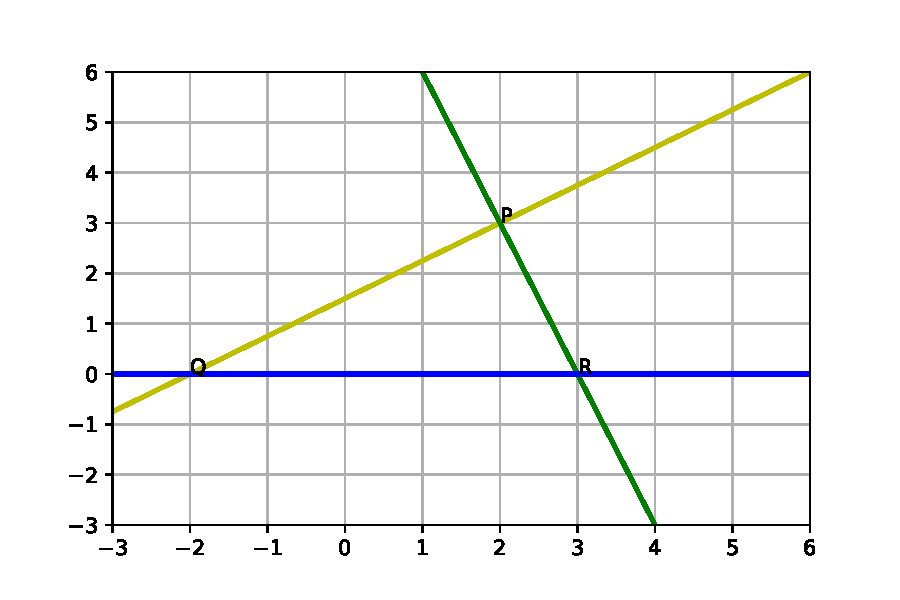
\includegraphics[width=8cm]{line.pdf}
\caption{Two lines representing given equations meet at point $\myvec{2 & 3}$ }.
\end{figure}
\item 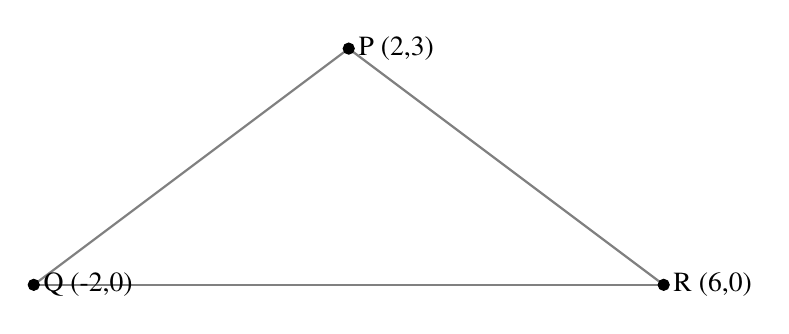
\begin{tikzpicture}
\draw[gray, thick] (-2,0) -- (2,3);
\draw[gray, thick] (6,0) -- (2,3);
\draw[gray, thick] (-2,0) -- (6,0);
\filldraw[black] (2,3) circle (2pt) node[anchor=west] {P (2,3)};
\filldraw[black] (-2,0) circle (2pt) node[anchor=west] {Q (-2,0)};
\filldraw[black] (6,0) circle (2pt) node[anchor=west] {R (6,0)};
\end{tikzpicture}
\begin{center}
    Tikz-Diagram
\end{center}
\end{enumerate}
\end{enumerate}
\end{document}
